\chapter*{Lista 3}
\addcontentsline{toc}{chapter}{Lista 3}


\subsection*{Zadanie 25}
\addcontentsline{toc}{section}{Zadanie 25}
Wykazać, że zmienna losowa $ X $ jest niezależna od $ \sigma $-algebry $ \mathcal B $ wtedy i tylko wtedy, gdy dla dowolnej funkcji borelowskiej ograniczonej $ \varphi $ takiej, że $ \mathbb E \left|\varphi(X)\right|<\infty  $ spełniony jest warunek
\begin{gather*}
\mathbb E \left(\varphi(X)|\mathcal B\right)=\mathbb E \varphi(X)
\end{gather*}

Rozwiązanie:
\begin{itemize}
\item $ \mathcal B=\sigma\left(A_1,A_2,\dots\right) $
\end{itemize}
"$ \Rightarrow $"
\begin{align*}
&\mathbb E \left(\varphi(X)|\mathcal B\right)
=\\=&
\sum_{i\in \mathbb N ,P\left(A_i\right)>0}
\mathbb E \left(\varphi(X)|\mathcal A_i\right)I_{A_i}
\stackrel{\Perp}{=}\\=&
\sum_{i\in \mathbb N ,P\left(A_i\right)>0}
\mathbb E \varphi(X)I_{A_i}
=\\=&
E\varphi(X)
\end{align*}
"$ \Leftarrow $" Dowód przez sprzeczność
\begin{align*}
\exists_{i\in \mathbb N }\mathbb E \left(\varphi(X)|\mathcal A_i\right)&\neq\mathbb E \left(\varphi(X)\right)\\
\sum_{i\in \mathbb N ,P\left(A_i\right)>0}
\mathbb E \left(\varphi(X)|\mathcal A_i\right)I_{A_i}&\neq
\sum_{i\in \mathbb N ,P\left(A_i\right)>0}
\mathbb E \varphi(X)I_{A_i}\\
\mathbb E \left(\varphi(X)|\mathcal B\right)&\neq
\mathbb E \varphi(X)
\end{align*}
czyli, $ \varphi(X) $ i $ A_i $ są zależne dla ustalonego $ i $, a tym samym $ \varphi(X) $ i $ \mathcal B $ są zależne. Czyli z prawa kontrapozycji zachodzi implikacja przeciwna.


\subsection*{Zadanie 31}
\addcontentsline{toc}{section}{Zadanie 31}
Niech dwuwymiarowy wektor losowy $ (X,Y) $ ma gęstość
\begin{gather*}
f(x,y)=\left \{
\begin{array}{lll}
	\frac{1}{\pi} & \text{dla} & x^2+y^2<1   \\
	0             & \text{dla} & x^2+y^2\ge1
\end{array}
\right .
(x,y)\in \mathbb R ^2
\end{gather*}
Wyznaczyć $ F_{X|Y} $ oraz obliczyć Cov$ (X,Y) $

Rozwiązanie:
\begin{align*}
&f_{X|Y}=\frac{f(x,y)}{\int\limits_{\mathbb R }f(x,y)\,dx}
=\\=&
\frac{1}{\pi}\mathbbm1_{\left\{x^2+y^2<1\right\}}(x,y)
\left(\int\limits_{-\sqrt{1-y^2}}^{\sqrt{1-y^2}}\frac{1}{\pi}\,dx\right)^{-1}
=\\=&
\frac{1}{\pi}\mathbbm1_{\left\{x^2+y^2<1\right\}}(x,y)\cdot
\frac{\pi}{2\sqrt{1-y^2}}
=\\=&
\frac{1}{2\sqrt{1-y^2}}\mathbbm1_{\left\{x^2+y^2<1\right\}}(x,y)
\end{align*}
\begin{align*}
\mathbb E Y=
\int\limits_{-1}^{1}\frac{y}{\pi}\cdot\frac{1}{2\sqrt{1-y^2}}\,dy=0
\end{align*}
\begin{align*}
\mathbb E XY=
\iint\limits_{x^2+y^2<1}\frac{xy}{\pi}\,dxdy=0
\end{align*}
\begin{gather*}
\text{Cov}(X,Y)=\mathbb E XY-\mathbb E X\mathbb E Y=0
\end{gather*}


\subsection*{Zadanie 32}
\addcontentsline{toc}{section}{Zadanie 32}
Niech dwuwymiarowy wektor losowy $ (X,Y) $ ma gęstość postaci:
\begin{gather*}
f(x,y)=\left \{
\begin{array}{cll}
	cx(2-2y-x) & \text{dla} & x,y>0\wedge \tfrac{x}{2}+y\le 1 \\
	0          & \text{dla} & \text{pzozstałe }x,y
\end{array}
\right .
\qquad (x,y)\in \mathbb R ^2
\end{gather*}
\begin{enumerate}[(i)]
\item Wyznaczyć stałą $ c $.
\item Obliczyć gęstości brzegowe $ f_X $ i $ f_Y $.
\item Wyznaczyć gęstości warunkowe $ f_{X|Y} $ i $ f_{Y|X} $.
\item Obliczyć warunkowe wartości oczekiwane $ \mathbb E \left(X|Y=y\right) $ i $ \mathbb E \left(Y|X=x\right) $.
\item Obliczyć warunkowe wariancje $ \Var \left(X|Y=y\right) $ i $ \Var \left(Y|X=x\right) $
\end{enumerate}

Rozwiązanie:
\begin{enumerate}[(i)]
\item 
\begin{align*}
&\int\limits_{0}^{1}\int\limits_{0}^{2-2y}cx(2-2y-x)\,dxdy
=\\=&
\int\limits_{0}^{1}\int\limits_{0}^{2-2y}c x (2-2y)-c x^2\,dxdy
=\\=&
\int\limits_{0}^{1}c\left(2-2y\right)\cdot\frac{\left(2-2y\right)^2}{2}-c\cdot\frac{\left(2-2y\right)^3}{3}\,dy
=\\=&
\int\limits_{0}^{1}c\left(1-y\right)^3\cdot \frac{8}{6}\,dy
=
\frac{c}{3}
\end{align*}
$ c=3 $
\item 
\begin{align*}
&f_X(x)
=
\int\limits_{0}^{1-\frac{x}{2}}3x(2-2y-x)\,dy
=\\=&
\int\limits_{0}^{1-\frac{x}{2}}3 (2-x) x-6 x y\,dy
=\\=&
\frac{3 x^3}{4}-3 x^2+3 x
\end{align*}
\begin{align*}
&f_Y(y)
=
\int\limits_{0}^{2-2y}3x(2-2y-x)\,dx
=\\=&
\int\limits_{0}^{2-2y}3 (2-x) x-6 x y\,dy
=\\=&
-4 (y-1)^3
\end{align*}
\item 
\begin{multicols}{2}
\begin{gather*}
f_{X|Y}
=
\frac{f(x,y)}{f_Y(y)}
\end{gather*}
\begin{align*}
&f_{X|Y}(x)
=\\=&
\frac{3x(2-2y-x)}{-4 (y-1)^3}
\end{align*}
\\
\begin{gather*}
f_{Y|X}
=
\frac{f(x,y)}{f_X(x)}
\end{gather*}
\begin{align*}
&f_{X|Y}(x)
=\\=&
\frac{3x (2-2y-x)}{\frac{3 x^3}{4}-3 x^2+3 x}
=\\=&
-\frac{4 (x+2 y-2)}{(x-2)^2}
\end{align*}
\end{multicols}
\item 
\begin{minipage}[t]{0.5\textwidth}
\begin{align*}
&\mathbb E \left(X|Y=y\right)
=\\=&
\int\limits_{0}^{2-2y}
x\cdot\frac{3x(2-2y-x)}{-4 (y-1)^3}
\,dx
=\\=&
\int\limits_{0}^{2-2y}
\frac{3 x^3}{4 (y-1)^3}+\frac{3 x^2}{2 (y-1)^2}
\,dx
=\\=&
1-y
\end{align*}
\end{minipage}
\begin{minipage}[t]{0.5\textwidth}
\begin{align*}
&\mathbb E \left(Y|X=x\right)
=\\=&
\int\limits_{0}^{1-\frac{x}{2}}
-y\cdot \frac{4 (x+2 y-2)}{(x-2)^2}
\,dy
=\\=&
\int\limits_{0}^{1-\frac{x}{2}}
-\frac{8 y^2}{(x-2)^2}-\frac{4 y}{x-2}
\,dy
=\\=&
\frac{2-x}{6}
\end{align*}
\end{minipage}
\item 
\begin{minipage}[t]{0.5\textwidth}
\begin{align*}
&\mathbb E \left(X|Y=y\right)^2
=\\=&
\int\limits_{0}^{2-2y}
x^2\cdot\frac{3x(2-2y-x)}{-4 (y-1)^3}
\,dx
=\\=&
\int\limits_{0}^{2-2y}
\frac{3 x^4}{4 (y-1)^3}+\frac{3 x^3}{2 (y-1)^2}
\,dx
=\\=&
\frac{6}{5} (y-1)^2
\end{align*}
\begin{align*}
&\Var\left(X|Y=y\right)
=\\=&
\frac{6}{5} (y-1)^2-\left(1-y\right)^2
=\\=&
\frac{1}{5} (y-1)^2
\end{align*}
\end{minipage}
\begin{minipage}[t]{0.5\textwidth}
\begin{align*}
&\mathbb E \left(Y|X=x\right)
=\\=&
\int\limits_{0}^{1-\frac{x}{2}}
-y\cdot \frac{4 (x+2 y-2)}{(x-2)^2}
\,dy
=\\=&
\int\limits_{0}^{1-\frac{x}{2}}
-\frac{8 y^3}{(x-2)^2}-\frac{4 y^2}{x-2}
\,dy
=\\=&
\frac{1}{24} (x-2)^2
\end{align*}
\begin{align*}
&\Var\mathbb E \left(Y|X=x\right)
=\\=&
\frac{1}{24} (x-2)^2-\left(\frac{2-x}{6}\right)^2
=\\=&
\frac{1}{72} (x-2)^2
\end{align*}
\end{minipage}
\end{enumerate}


\subsection*{Zadanie 33}
\addcontentsline{toc}{section}{Zadanie 33}
Wyznaczyć gęstość wektora losowego $ X,Y $, jeśli gęstość brzegowa $ f_X $ jest postaci
\begin{gather*}
f_X(x)=\left \{
\begin{array}{cll}
	c(x-2)^2  & \text{dla} & 2<x\le 7           \\
	c(12-x)^2 & \text{dla} & 7<x\le 12          \\
	    0     & \text{dla} & \text{pozostałe } x
\end{array}
\right .
\qquad x\in \mathbb R 
\end{gather*}
dla pewnej stałej $ c $ oraz dana jest gęstość brzegowa $ f_{Y|X} $ postaci
\begin{gather*}
f_{Y|X}(y|x)=\left \{
\begin{array}{cll}
	\frac{1}{3} & \text{dla} & \frac{x}{2}-1\le y\le\frac{x}{2}+2 \\
	     0      & \text{dla} & \text{else}
\end{array}
\right .
\qquad y\in \mathbb R , x\in(2,12)
\end{gather*}

Rozwiązanie:
\begin{gather*}
\int\limits_{2}^{12}f_X(x)\,dx=1
\end{gather*}
\begin{align*}
&\int\limits_{2}^{12}f_X(x)\,dx
=\\=&
\int\limits_{2}^{7}c(x-2)^2\,dx
+
\int\limits_{7}^{12}c(12-x)^2\,dx
=\\=&
\frac{250 c}{3}=1
\end{align*}
$ c=\frac{3}{250} $
\begin{align*}
f_{Y|X}(y|x)
=&
\frac{f_{X,Y}(x,y)}{f_X(x)}
\\
f_{Y|X}(y|x)f_X(x)
=&
f_{X,Y}(x,y)
\end{align*}
\begin{align*}
&\frac{1}{3}\mathbbm1_{\left[\frac{x}{2}-1,\frac{x}{2}+2\right]}(y)\cdot
\left(
\frac{3}{250}(x-2)^2\mathbbm1_{(2,7]}(x)
+
\frac{3}{250}(12-x)^2\mathbbm1_{(7,12]}(x)
\right)
=\\=&
\frac{1}{250}
\left((x-2)^2\mathbbm1_{(2,7]}(x)\mathbbm1_{\left[\frac{x}{2}-1,\frac{x}{2}+2\right]}(y)
+
(12-x)^2\mathbbm1_{(7,12]}(x)\mathbbm1_{\left[\frac{x}{2}-1,\frac{x}{2}+2\right]}(y)\right)
\end{align*}


\subsection*{Zadanie 34}
\addcontentsline{toc}{section}{Zadanie 34}
Wektor losowy $ (X,Y) $ ma gęstość
\begin{gather*}
f(x,y)=\left \{
\begin{array}{cll}
	x+y & \text{dla} & (x,y)\in[0,1]    \\
	 0  & \text{dla} & (x,y)\notin[0,1]
\end{array}
\right .
\qquad (x,y)\in \mathbb R ^2
\end{gather*}
Wyznaczyć $ \mathbb E \left(X|Y=y\right) $ oraz $ \mathbb E \left(X\exp \left(Y+\frac{1}{Y}\right)|Y=y\right) $

Rozwiązanie:
\begin{gather*}
f_{X|Y}(x,y)
=
\frac{f_{X,Y}(x,y)}{f_Y(y)}
\end{gather*}
\begin{align*}
f_Y(y)
=&
\int\limits_{\mathbb R }f_{X,Y}(x,y)\,dx
=\\=&
\int\limits_{0}^{1}x+y\,dx=y+\frac{1}{2}
\end{align*}
\begin{gather*}
f_{X|Y}(x,y)
=
\frac{x+y}{y+\frac{1}{2}}=\frac{2x+2y}{2y+1}
\end{gather*}
\begin{align*}
\mathbb E \left(X|Y=y\right)=&
\int\limits_{0}^{1}
x\cdot\frac{2x+2y}{2y+1}
\,dx
=\\=&
\int\limits_{0}^{1}
\frac{2 x^2}{2 y+1}+\frac{2 x y}{2 y+1}
\,dx
=\\=&
\frac{2}{3 (2 y+1)}+\frac{y}{2 y+1}
=\\=&
\frac{3 y+2}{6 y+3}
\end{align*}
Własność
\begin{gather*}
\mathbb E \left(X\varphi(Y)|Y\right)
=
\varphi(Y)\mathbb E \left(X|Y\right)
\end{gather*}
Stosujemy
\begin{align*}
&\mathbb E \left(X\exp \left(Y+\tfrac{1}{Y}\right)|Y=y\right)
=\\=&
\exp \left(y+\tfrac{1}{y}\right)\mathbb E \left(X|Y=y\right)
=\\=&
\exp \left(y+\tfrac{1}{y}\right)\frac{3 y+2}{6 y+3}
\end{align*}
%
%
%\addcontentsline{toc}{section}{Zadanie 35}
%\subsection*{Zadanie 35}Niech dwuwymiarowy wektor losowy $ (X,Y) $ ma gęstość
%\begin{gather*}
%f(x,y)=\left \{
%\begin{array}{cll}
%	c(|x|+|y|) & \text{dla} & (x,y)\in K    \\
%	    0      & \text{dla} & (x,y)\notin K
%\end{array}
%\right .
%\qquad (x,y)\in \mathbb R ^2
%\end{gather*}
%gdzie $ K\subset \mathbb R ^2 $ jest równoległobokiem ograniczonym prostymi:\\
%$ y=x-1\\
%y=x+1\\
%y=\frac{x}{3}-1\\
%y=\frac{x}{3}+1 $.\\
%Wyznaczyć stałą $ c $ oraz $ \mathbb E \left(X|Y=y\right), \mathbb E \left(X^2|Y=y\right),\mathbb E \left(Y|X=x\right) $.
%
%Rozwiązanie:
%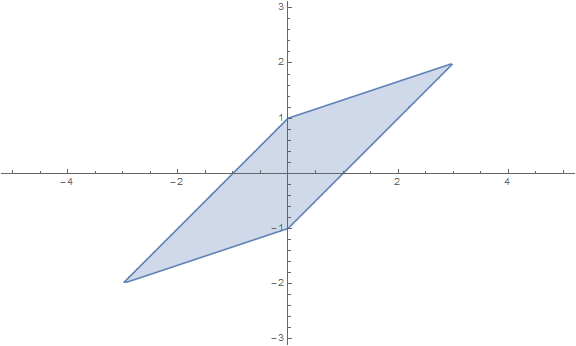
\includegraphics[width=0.7\linewidth]{Region1}\\
%\begin{align*}
%&\int\limits_{K}f(x,y)\,dxdy
%=\\=&
%\int\limits_{-\frac{5}{2}}^{\frac{5}{2}}\int\limits_{\frac{x}{3}-1}^{x+1}f(x,y)\,dydx
%+
%\int\limits_{-\frac{5}{2}}^{\frac{5}{2}}\int\limits_{x-1}^{\frac{x}{3}+1}f(x,y)\,dydx
%=\\=&
%2\int\limits_{0}^{\frac{5}{2}}\int\limits_{x-1}^{\frac{x}{3}+1}c(x+|y|)\,dydx
%\end{align*}


\subsection*{Zadanie 36}
\addcontentsline{toc}{section}{Zadanie 36}
Dwuwymiarowy wektor losowy $ (X,Y) $ ma gęstość
\begin{gather*}
f(x,y)=\left \{
\begin{array}{cll}
	0,2(x+2y) & \text{dla} & (x,y)\in[0,1] \times [0,2]   \\
	    0     & \text{dla} & (x,y)\notin[0,1]\times [0,2]
\end{array}
\right .
\qquad (x,y)\in \mathbb R ^2
\end{gather*}
Wyznaczyć:\\
$ \mathbb E \left(X|Y=y\right)\\
\mathbb E \left(X^2+1|Y=y\right) \\
\mathbb E \left(Y|X=x\right)$

Rozwiązanie:\\
\begin{minipage}[t]{0.5\linewidth}
\begin{align*}
&f_{X|Y}(x|y)
=\\=&
\frac{f(x,y)}{f_Y(y)}
=\\=&
\frac{\frac{1}{5}(x+2y)}{\int\limits_{0}^{1}\frac{1}{5}(x+2y)\,dx}
=\\=&
\frac{2(x+2y)}{4 y+1}
\end{align*}
\begin{align*}
&\mathbb E \left(X|Y=y\right)
=\\=&
\int\limits_{0}^{1}x\cdot \frac{2(x+2y)}{4 y+1}\,dx
=\\=&
\int\limits_{0}^{1}\frac{2 x^2}{4 y+1}+\frac{4 x y}{4 y+1}\,dx
=\\=&
\frac{6 y+2}{12 y+3}
\end{align*}
\end{minipage}
\begin{minipage}[t]{0.5\linewidth}
\begin{align*}
&f_{Y|X}(y|x)
=\\=&
\frac{f(x,y)}{f_X(x)}
=\\=&
\frac{\frac{1}{5}(x+2y)}{\int\limits_{0}^{2}\frac{1}{5}(x+2y)\,dy}
=\\=&
\frac{(x+2y)}{2 (x+2)}
\end{align*}
\begin{align*}
&\mathbb E \left(Y|X=x\right)
=\\=&
\int\limits_{0}^{2}y\cdot \frac{(x+2y)}{2 (x+2)}\,dy
=\\=&
\int\limits_{0}^{2}\frac{y^2}{x+2}+\frac{x y}{2 x+4}\,dy
=\\=&
\frac{3 x+8}{3 x+6}
\end{align*}
\end{minipage}\\
\begin{align*}
&\mathbb E \left(X^2+1|Y=y\right)
=\\=&
\int\limits_{0}^{1}
(x^2+1)\cdot\frac{2(x+2y)}{4 y+1}
\,dx
=\\=&
\int\limits_{0}^{1}
x^2\cdot\frac{2(x+2y)}{4 y+1}
\,dx
+
\cancelto{1}{\int\limits_{0}^{1}
\frac{2(x+2y)}{4 y+1}
\,dx}
=\\=&
\int\limits_{0}^{1}
\frac{2 x^3}{4 y+1}+\frac{4 x^2 y}{4 y+1}
\,dx
+1
=\\=&
\frac{32 y+9}{24 y+6}
\end{align*}